\documentclass[11pt, oneside]{article}   	% use "amsart" instead of "article" for AMSLaTeX format
%\usepackage{geometry} 
\usepackage[margin=0.8in]{geometry}                		
\geometry{letterpaper}                   		% ... or a4paper or a5paper or ... 
%\geometry{landscape}                		% Activate for rotated page geometry
%\usepackage[parfill]{parskip}    		% Activate to begin paragraphs with an empty line rather than an indent
\usepackage{graphicx}				% Use pdf, png, jpg, or eps§ with pdflatex; use eps in DVI mode
								% TeX will automatically convert eps --> pdf in pdflatex		

\usepackage{amssymb}
\usepackage{hyperref}
\usepackage{tabularx}
\hypersetup{
    colorlinks=true,
    linkcolor=blue,
    filecolor=blue,      
    urlcolor=blue,
    }
%SetFonts

%SetFonts
%\vspace{-5ex}

\graphicspath{ {./images/} }


\title{Group 1: Smart City Lights}

\author{
    Deepak Mathur  \qquad   
    Ashee Jain  \qquad
    Srujana Sabbani  \\
    Atanu Kar \qquad
    Anjali Manoj \\ 
   22111019, 22111073, 22111083, 22111086, 22111262\\
   {\tt \{deepakm22, asheejain22, srujanas22, atanukar22, anjalim22\}@iitk.ac.in}\\
{Indian Institute of Technology Kanpur (IIT Kanpur)}
}


\date{}							% Activate to display a given date or no date

\begin{document}

\maketitle

\abstract{A Smart City is a technologically advanced urban area that uses various electronic methods to manage and improve all operations. In the current situation, streetlights are switched on during the night and off during the day, Light Emitting Diodes (LED) are used to save energy consumption, and also, fault detection in LEDs is done manually which can lead to a delay in fixing them. These problems are addressed in this project using the Internet of Things (IoT). The idea is about designing and implementing an automated street lighting system on public roads, mainly focusing on avoiding energy wastage and having proper maintenance support for the implemented system. Our proposed system makes use of Passive Infrared sensor (PIR) sensors to detect vehicle motion and regulate the intensity of LED lights for energy saving. It also uses Light Dependent Resistors (LDR), and a Global Positioning System (GPS) module to monitor the LED functionality and report any fault and its corresponding location respectively, thus creating a robust system. All these communications happen over Long Range (LoRa) communication protocol via a gateway. Hence, this system could be implemented in real-time for energy-saving by controlling the streetlights on the road networks.}
    
\section{Introduction}
In India, there are more than 27 million lamp posts that are used to light up the streets. This demands a huge amount of electricity anywhere between 20 - 40\% of 
the energy produced in India. Initially, CFL, metal halides, or sodium vapor lights were used in lamp posts, but to save energy, the government has come up with LEDs 
to be installed on lamp posts. In the current scenario, streetlights are automatically switched on at night around 6:00 pm and switched off in the mornings around 
06:00 am. This leads to a lot of energy usage for 12 hours. Usually, when a lamp post stops working, its status is either informed by the neighboring people to the concerned 
office or manually done by the electricity inspectors frequently in their assigned area. This makes the maintenance of streetlights a delayed process, involving human 
intervention. These statistics on the consumption of electricity on streetlights and delayed, human-intervened maintenance shows that there is a need for an automated smart
street lighting system that aims at reducing power consumption and improving fault detection.
Ian n this project, a lamp post is made smart by adding Arduino Uno, a microcontroller, and sensors such as PIR and LDR, GPS. LoRa, which is a low-cost, long-range communication protocol, is used in this project. Its features are anti-interference capability, spread-spectrum, wide-coverage, wireless, and security. 

This paper is organized into the following sections: research work referenced in section 2, the proposed architecture in section 3, the implementation and flow of the proposed idea 
in section 4, results in section 5, future work and improvements in section 6, the conclusion of the project in section 7, and the contribution of each member in section 8.



\section{Related Work}
The main objective of this paper \cite{1} is to identify faulty streetlights by using illumination maps (IMaps). The faulty streetlights are based on the difference in the illumination intensity at 
location 'q' between the two iMaps taken at $time_1$ and $time_2$. This data on IMaps is collected by Hitchhiker installed on taxis and shuttle vans. This paper \cite{2} proposes the idea to use LDR and a real-time clock to control the LEDs on the lamp post. Also, based on the vehicle's speed and time of the day, the LEDs intensity is regulated using a 
light-dimming circuit. It also implemented fault detection by identifying the faulty LED and sending its location to an android application. This paper \cite{3} involves creating a network of nodes that can easily accept new nodes and scale up the network without affecting the existing network. It also involves the use of a PIR sensor to detect 
vehicle movement and passes the info to the gateway in case any fault is detected. The idea proposed in this paper \cite{4} is about controlling the intensity of light based on users on the road and the surroundings light. If the LDR detects sunlight below 80\%, the LEDs are turned. 
Similarly, two IR sensors are used to detect the motion and the speed of the vehicle to regulate the intensity of light. This paper \cite{5} considered both directions of the road and vehicle motion to provide sufficient lighting ahead of the vehicle without violating the lighting rules of the road. This paper \cite{6} also extended to 
consider the pedestrian walk on both sides of the road when considering the lamp post automation. The approach used in this paper6 is to low-cost sensors and a control system to send information. It also does adaptive street lighting using this information.
This paper \cite{7} involves using Arduino Uno and sensors for motion detection and light from the environment to decide whether the LED street light needs to switch on or off and regulate the intensity of
 light. This paper \cite{8} involves using two LDRs, one to monitor LED and another to sense light from the environment and based on the value of LDRs to detect the fault of LED. Here, the Xbee transmission module 
transfers the data to Arduino Uno. This also uses the idea of dimming the streetlights based on the users available. This paper \cite{9} involves Zigbee-based communication between sensor nodes to pass the info from node to node and uses a cellular network to transfer the info to base stations or servers.
This paper \cite{10} shows the concept of multi-hop communication gateway to gateway communication using LoRa.

The limitations that are identified from the above references are high implementation costs as each node has more sensors and hardware, the network design and implementation are complex, the 
maintenance of the Wireless Sensor Network (WSN) is costly and needs efforts constantly, all the references use short-range communication hence more nodes need to be installed. The advantages of 
this project over the existing systems are the proposed idea is a cost-friendly solution as it requires less number of nodes to control a set of LEDs around these nodes, the short-range communication 
protocols are replaced by LoRa, maintenance is easy and faster due to lesser nodes, this system can be deployed with the existing system, unlike others which replace the existing system.



\section{Proposed Idea}

The proposed idea of this project involves building a two-tier architecture, sensor node to gateway and gateway to server, over LoRa communication protocol. The gateway, based on Raspberry Pi, can also act as a node and the sensor nodes are based on Arduino UNO. There are PIR sensors at each node that detect the motion of any object that passes by and an LDR sensor that detects the fault. Here, we consider that a single node controls the functioning of 5 - 8 streetlights. Assuming each streetlight is at a distance of 70 m, one node covers approx. 350 - 560 m area. The initial node (Arduino/Raspberry Pi) detects an object, lights up the LEDs of the connected streetlights, and sends the information to the next node in line. The second one confirms the presence of the same object using PIR and with the information gained from the previous node, lights up the LED and this process continues. In case of a fault within the node-LED groups, the LDR placed at each streetlight detects it and sends this information, node ID, and accurate location using GPS to the gateway through LoRa, imploring immediate attention. 

Unlike the current scenario of automatic streetlights which uses communication protocols such as ZigBee and Bluetooth Low Energy (BLE), the protocol used here is LoRa in view of its long range and topology. LoRa has a star topology, implying direct communication with the gateway, which is mandatory with respect to the proposal. Comparatively, it has also got a lower cost and lower use of power. Moreover, LoRa also supports multi-channel gateway communication as well as RSSI-based localization, which makes it suitable for this project setting.


\section{Methodology}
\subsection{Architecture}
Our project has a two-tier architecture: Sensor node to Gateway and Gateway to server.
\begin{enumerate}
\item \textbf{Sensor node to Gateway:} The sensor node is equipped with PIR, LDR, and GPS sensors, on detecting motion the PIR sensor turns on all the LEDs connected to the sensor node, and the same information is sent over LoRa to the neighboring nodes. This constitutes the sensor node to sensor node communication. When the LDR connected to each LED/streetlight does not detect light during the night or it detects light during the day, such condition indicates the presence of a fault in the LED, and the node ID along with GPS location is sent to the nearest gateway server over LoRa.\\

\item \textbf{Gateway to server:} The gateway on receiving the fault information from the sensor nodes forwards it further to the server and/or the next gateway in case of direct connection loss. The gateway and the server communicate over Ethernet. If the connection between the server and a gateway becomes faulty, the same data is sent by another gateway to the server. This achieves fault tolerance. \\
\end{enumerate}


\subsection{Project Design}

In order to implement the project idea we started with the selection of hardware. We have used two separate IoT development boards i.e Arduino Uno and Raspberry Pi model 3B to configure them as sensor nodes\cite{11} . However, Raspberry Pi based sensor nodes are also configured as a gateway too. We have carried out the evaluation of the project where we had four Arduino-based sensor nodes and two Raspberry Pi based sensor nodes with Raspberry Pi also acting as gateways. We have used IC LM7805 in order to get a regulated output voltage of 5V. In order to detect vehicle movement we have used the PIR sensor of model HCSR 501 and for detection of LED working status, we have used LDR sensors which were placed with all the streetlights. During the night, if PIR detects any movement and LED is not working then the sensor node considers it as a fault. The GPS module connected to each Arduino Uno based sensor node gives the location of the sensor node so as to help the repair team carry out the repair work faster. The Raspberry Pi based nodes do not have any GPS module as we are considering that the location of all the gateways is fixed and updated in the database. Table \ref{tab:hardware} shows the details of hardware used in this project.



\begin{table}[h]
    \centering
    \begin{tabular}{|c|c|}
    \hline
    \textbf{Components} &  \textbf{Description}\\

    \hline
     Motion Detection & PIR sensor HCSR 501\\
     \hline        
    Fault Detection  &  LDR Sensor LM393 \\
    \hline
    Location         &   GPS Module GY-NE06MV2 \\
    \hline
    LoRa Module	& LoRa Ra-02 SX1278 433MHz\\
    \hline
    Dev Board	& Arduino UNO and Raspberry Pi 3 B \\
    \hline
    Voltage Regulator	& IC LM7805 \\
    \hline
    \end{tabular}
    \caption{Hardwares used}
    \label{tab:hardware}
\end{table}

 \begin{figure}[!h]
\centering
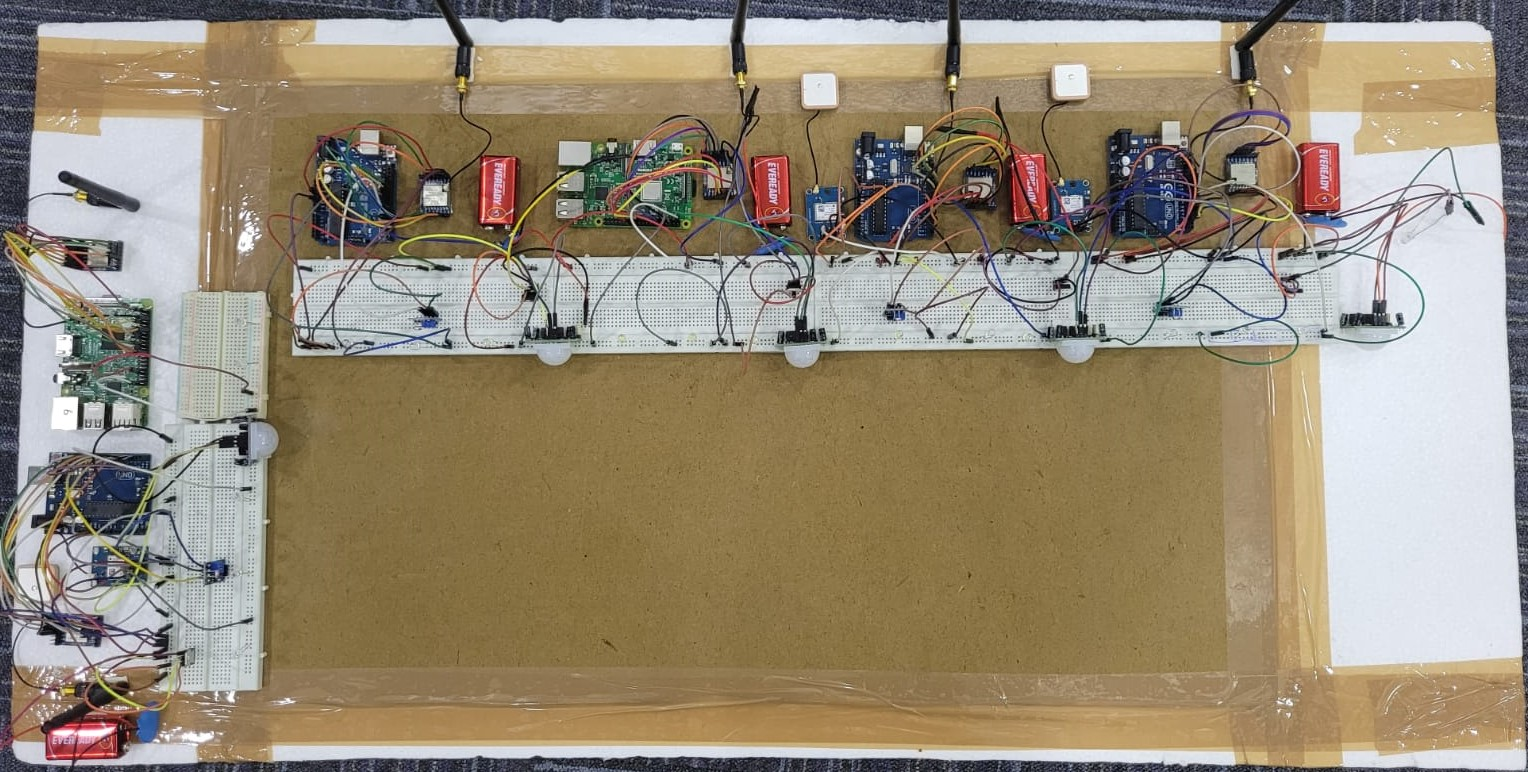
\includegraphics[scale=0.35]{images/complete_project_image.jpeg}
\caption{\centering Smart City-lighting prototype model}
\label{complete_model}
\end{figure}

In this project we have only shown (figure \ref{complete_model}) for one side of a four to six lane highway. As per the width of the road/highway potentiometer (sensitiity) of PIR sensor needs to be adjusted. We have taken into consideration while programming that if anybody takes an exit from the highway then the next PIR sensor would not detect any motion and thus LEDs placed ahead would not be turned on. The functioning of the project as per the data flow diagram given below can be implemented for the other side of the highway as well. Therefore our project is scalable. Security of the Nodes and gateways are discussed in section 4.4. In this project we hve considered that the distance between two sensor nodes will be 700-800 meter and the gap between two streetlight is 70-80 meters though the communication range between two LoRa nodes are much higher than that. The increase in gap between two Nodes will lead to more additional cabling and increase the repair time by homing on the faulty light.

\subsection{Data Flow Diagram}

In our project sensor data flows from bottom to top, unlike the directed fusion principle. In this, all sensor nodes keep passing the sensed information of object detection to its next sensor node over LoRa\cite{13}. For LoRa communication between Node to Node (Arduino UNO based) we had used LoRa header files taken from Sandeep Mistry \cite{14}. On receiving the information from the previous node it turns on a group of LEDs ahead of the node (for a particular area of responsibility). At any junction or round about sensor nodes deployed prior to that are responsible for turning ON the LEDs at the round about as well as two LEDs in each of the lane.   In case any fault is detected by LDR sensors placed on each streetlight, the sensor node initiates the GPS module and then the fault status along with the location information is passed to the gateway over LoRa \cite{12}. The gateway receives the payload, decodes, and applies a filter to take out relevant information i.e Node ID, Latitude value, and Longitude value. (Figure \ref{DFD}) given below describes how this information (Fault Status and Motion detection) is passed to gateway and sensor nodes. 

 \begin{figure}[h]
\centering
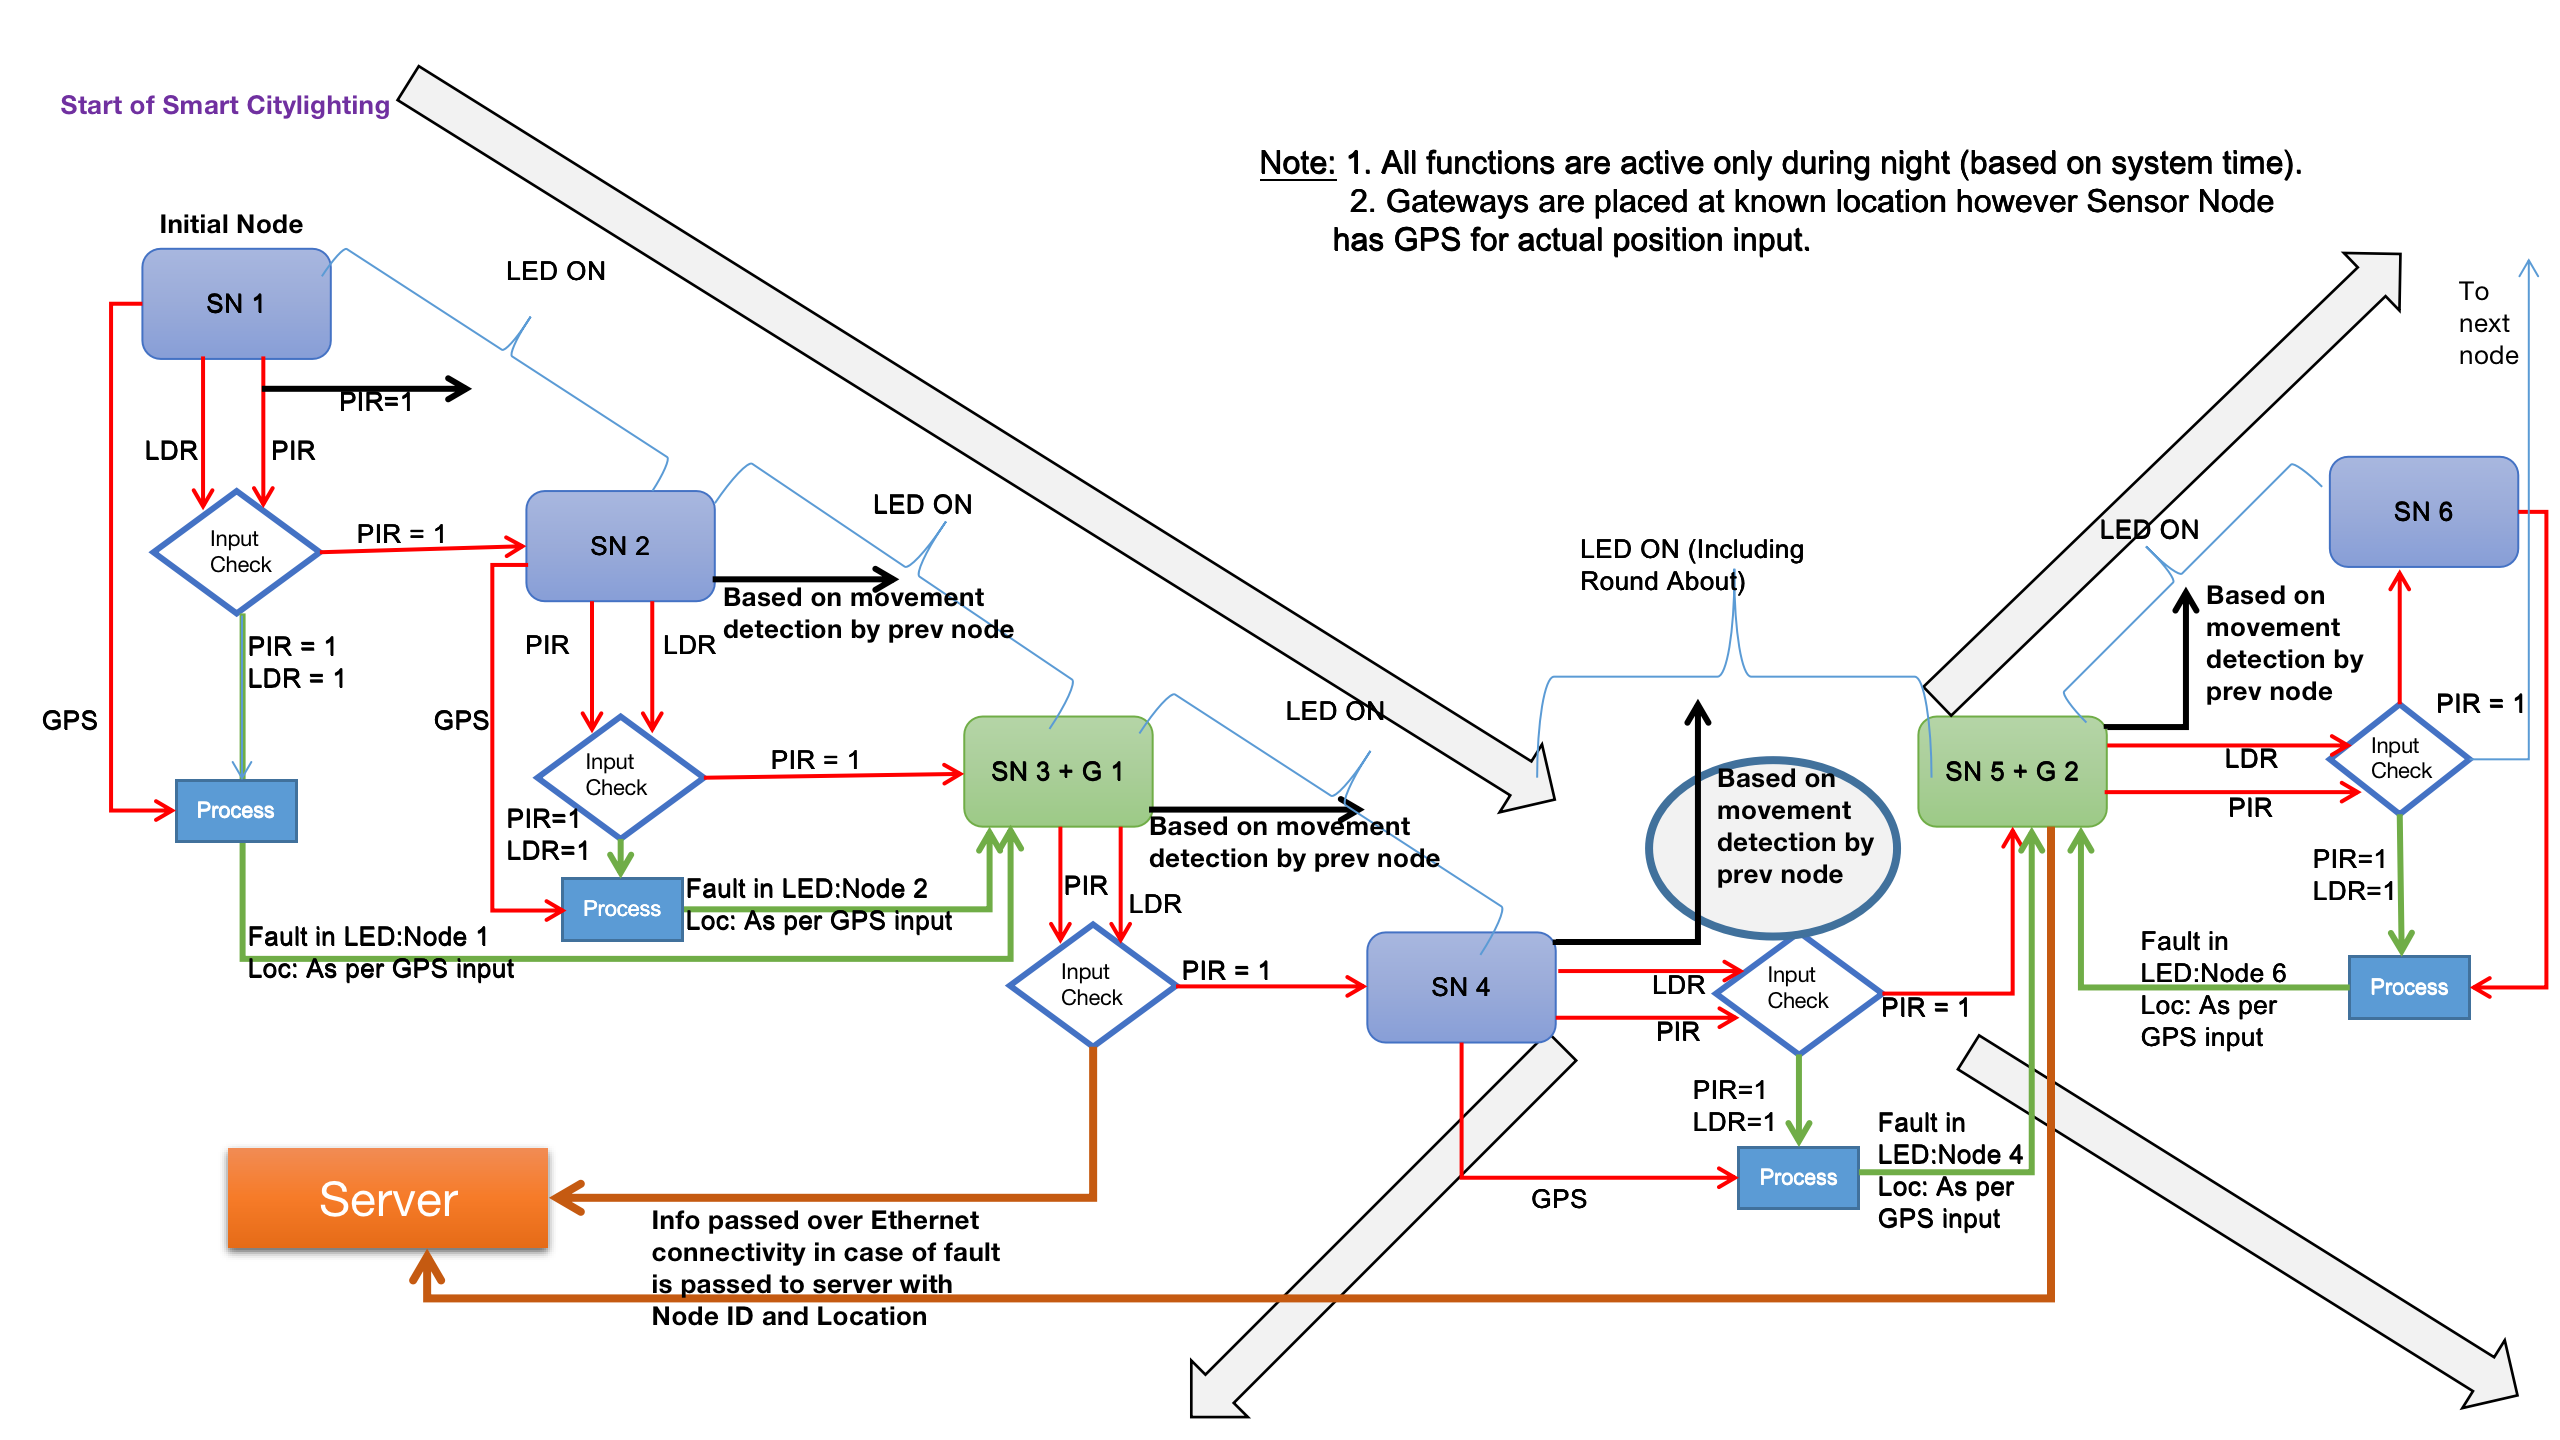
\includegraphics[scale=0.17]{images/DFD.png}
\caption{\centering Data Flow Diagram : Smart City-lighting}
\label{DFD}
\end{figure}

The gateway does two kinds of functioning, first, it sends the fault status along with location information to the server if the internet connectivity is proper. Secondly, it passes the information to the nearest gateway as well so as to achieve fault tolerance and multi-path routing. At the server end, the fault information passed by the gateway is received over the internet and displayed on a dashboard. The repair team can now go to the exact location of the fault to carry out repair work. Server/Cloud connectivity, Development of the dashboard, and adding of other features like Network/End Device Monitoring, and configuring firewalls are left to readers as per the requirement of project implementation in various different environments.


\subsection{Security}

In today’s world of increasing cyber-attacks on small IoT devices, maintaining security is very crucial in order to ensure data privacy and also for securing the functionality of the IoT system. We have achieved a secure login using credentials on the gateway node, which obstructs unauthorized access. Along with this, a packet filtering mechanism is also implemented which stops any arbitrary corrupted packet from making any change in the IoT system.\\

\section{Results}

The result of the different modules of this project is as follows: 
\begin{enumerate}
  \item The first module is node-to-node communication. Each node consists of a microcontroller i.e., Arduino Uno, a PIR sensor, an  LDR sensor, and a GPS module. These modules communicate over LoRa. The first node detects the motion (Figure \ref{module1-1}) of vehicles and sends a status 'HIGH' to Arduino Uno (Figure \ref{module1-3}). Now, based on the real-time clock, the LED lights following the first node are turned on (Figure \ref{module1-2}), and also, sends a signal to the next node so as to turn the controllable LEDs ahead of it on (Figure \ref{module1-4}).
  
  
  \begin{figure}[!ht]
  \centering
  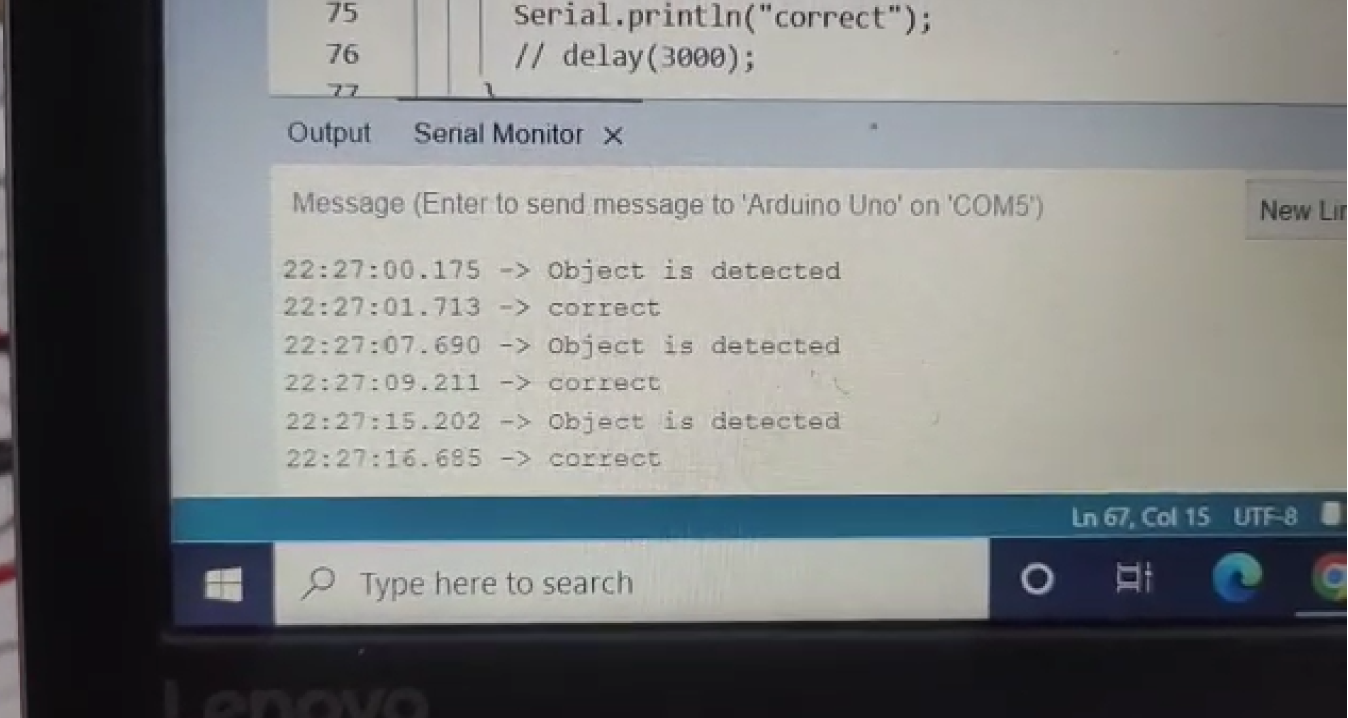
\includegraphics[width=0.5\textwidth]{images/module1-1.png}
  \caption{The PIR on the first node detecting the object's motion.}
  \label{module1-1}
  \end{figure}
  
  \begin{figure}[!ht]
  \centering
  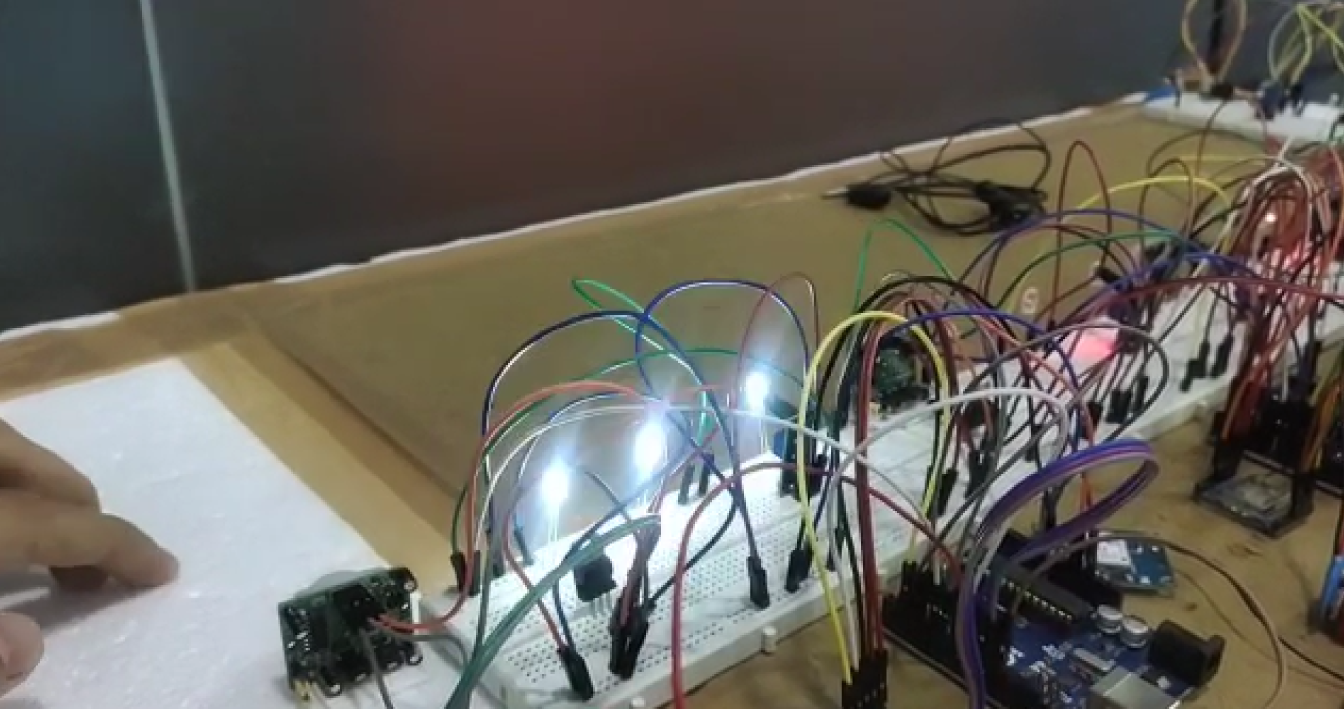
\includegraphics[width=0.5\textwidth]{images/module1-2.png}
  \caption{After the first node has detected the motion and it turns on the LEDs ahead of it.}
  \label{module1-2}
  \end{figure}
  
  \begin{figure}[!ht]
  \centering
  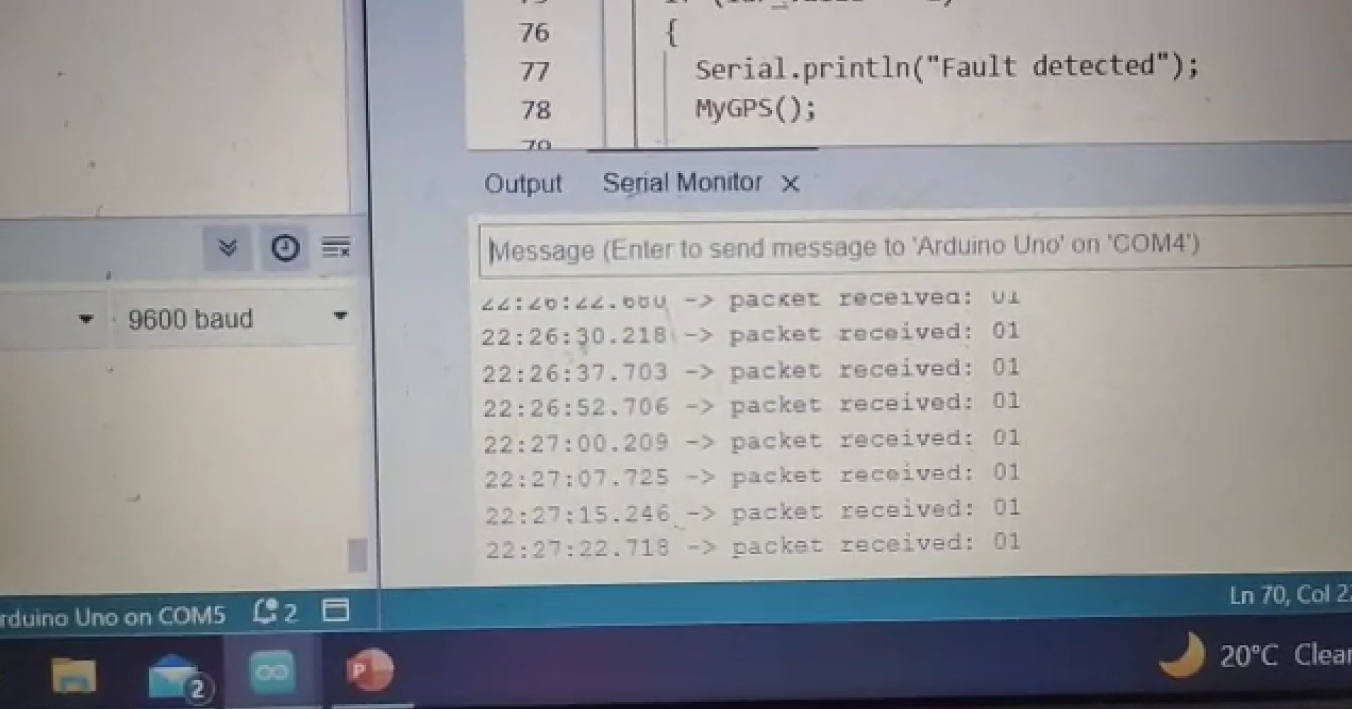
\includegraphics[width=0.5\textwidth]{images/module1-3.png}
  \caption{The PIR data of the first node is sent to the next nearest node. }
  \label{module1-3}
  \end{figure}
  
  \begin{figure}[!ht]
  \centering
  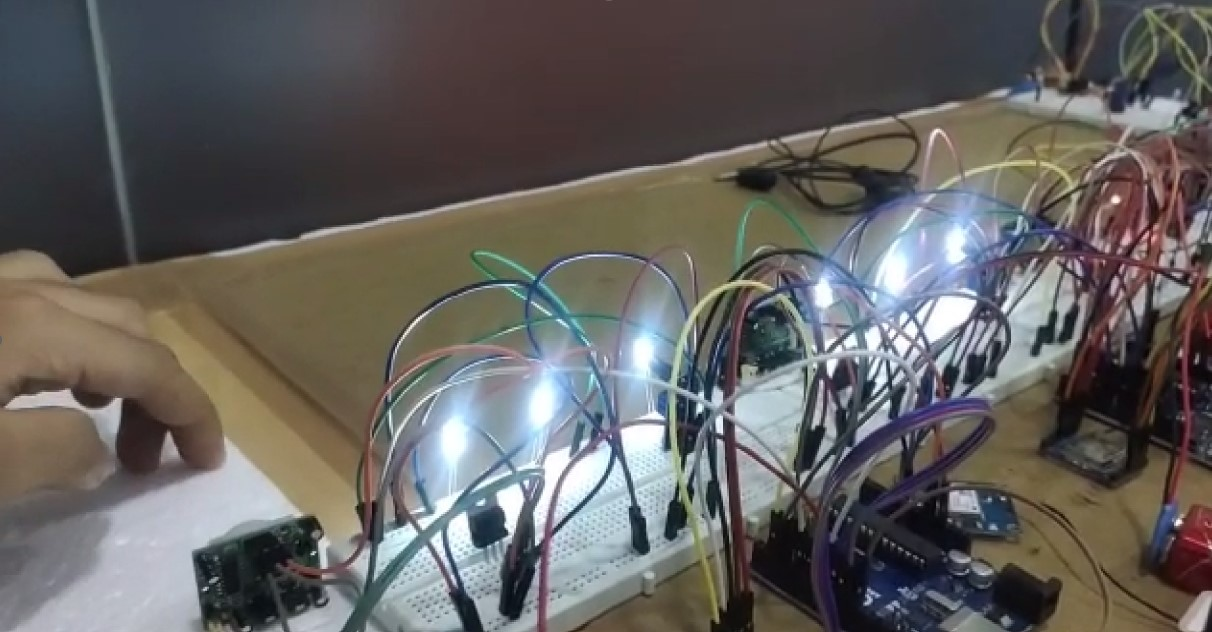
\includegraphics[width=0.5\textwidth]{images/module1-4.jpg}
  \caption{The next node on receiving data from the previous node, turns on LEDs ahead of it. }
  \label{module1-4}
  \end{figure}
  
  \item The second module is a node-to-gateway communication over LoRa. The gateway is implemented using Raspberry Pi. This communication involves sending the GPS location of the node (Figure \ref{module2-1}) that detects a fault in its controllable LEDs to the gateway as an alert (Figure \ref{module2-3}). This fault is detected by the LDR that is installed along with each LED to monitor it (Figure \ref{module2-2}).
  \begin{figure}[!ht]
  \centering
  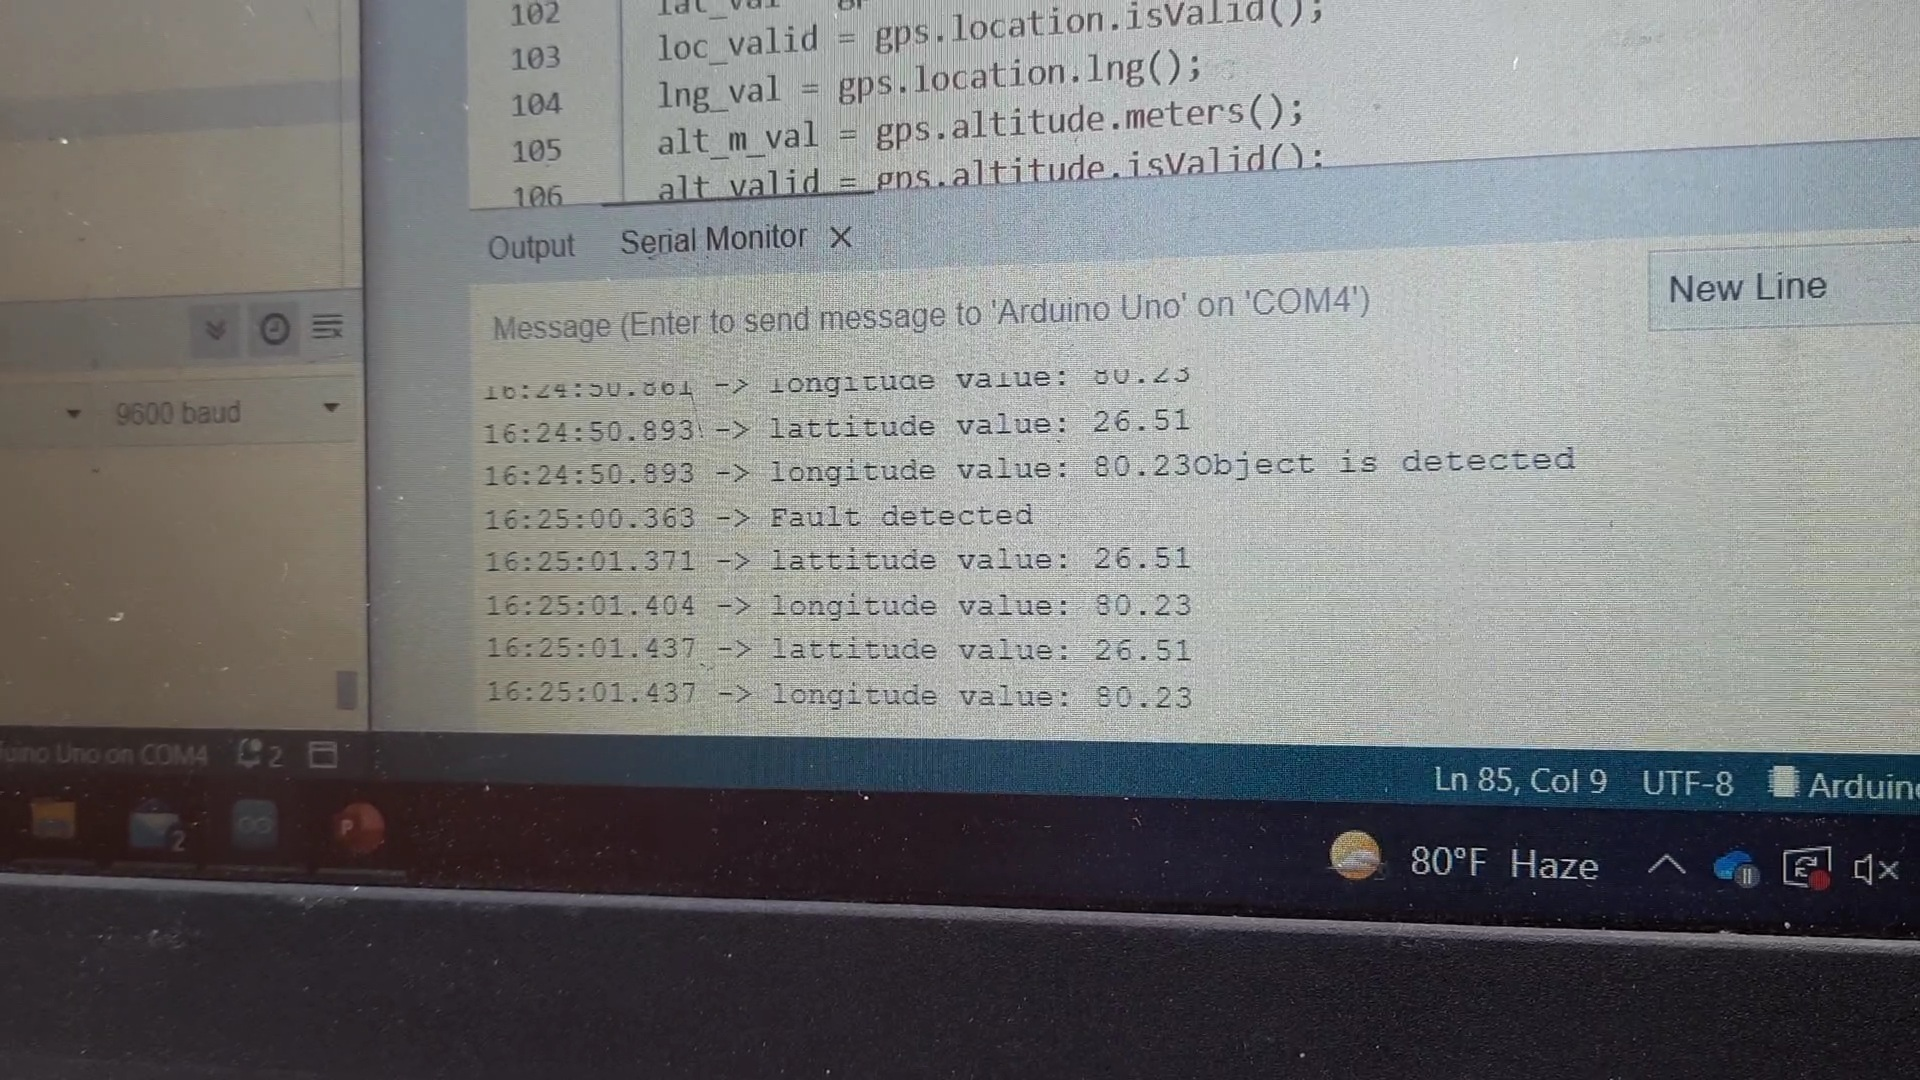
\includegraphics[width=0.5\textwidth]{images/module2-1.jpg}
  \caption{A fault is detected at the first node as the LED does not glow when an object is detected}
  \label{module2-1}
  \end{figure}
  
  \begin{figure}[!ht]
  \centering
  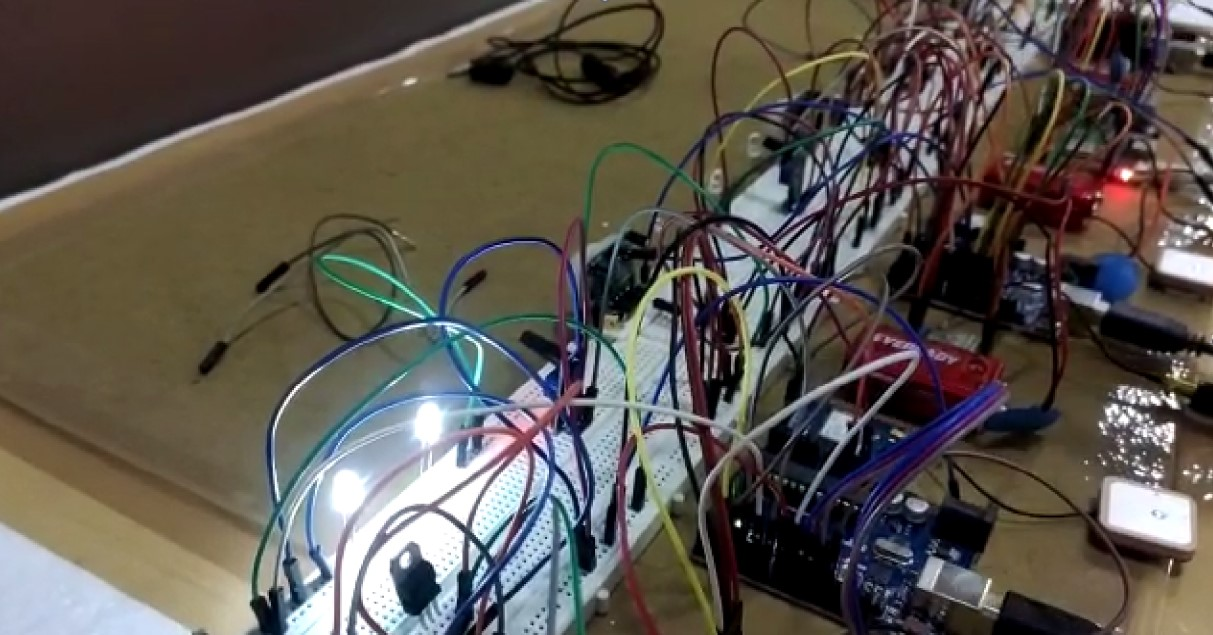
\includegraphics[width=0.5\textwidth]{images/module2-2.jpg}
  \caption{The node with no LED glowing near LDR. }
  \label{module2-2}
  \end{figure}
  
  \begin{figure}[!ht]
  \centering
  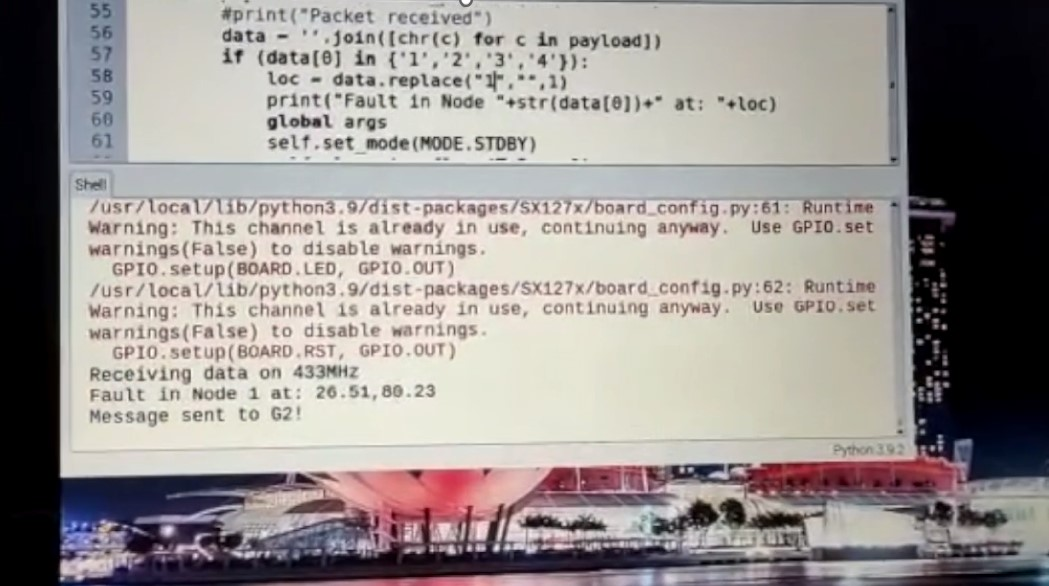
\includegraphics[width=0.5\textwidth]{images/module2-3.jpg}
  \caption{ The gateway receives the location of the faulty LED from node. }
  \label{module2-3}
  \end{figure}

  
\item The third module is the gateway to gateway communication over Lora. Here the information collected from nodes by the gateway is sent to the neighboring gateways (figure: \ref{module3-1}) and this process continues for multi-path routing and fault tolerance. This data is also sent to the server from the gateway over an Ethernet connection. If the connection between the server and a gateway becomes faulty, the same data is sent by another gateway to the server, thereby achieving fault tolerance.
\begin{figure}[!ht]
  \centering
  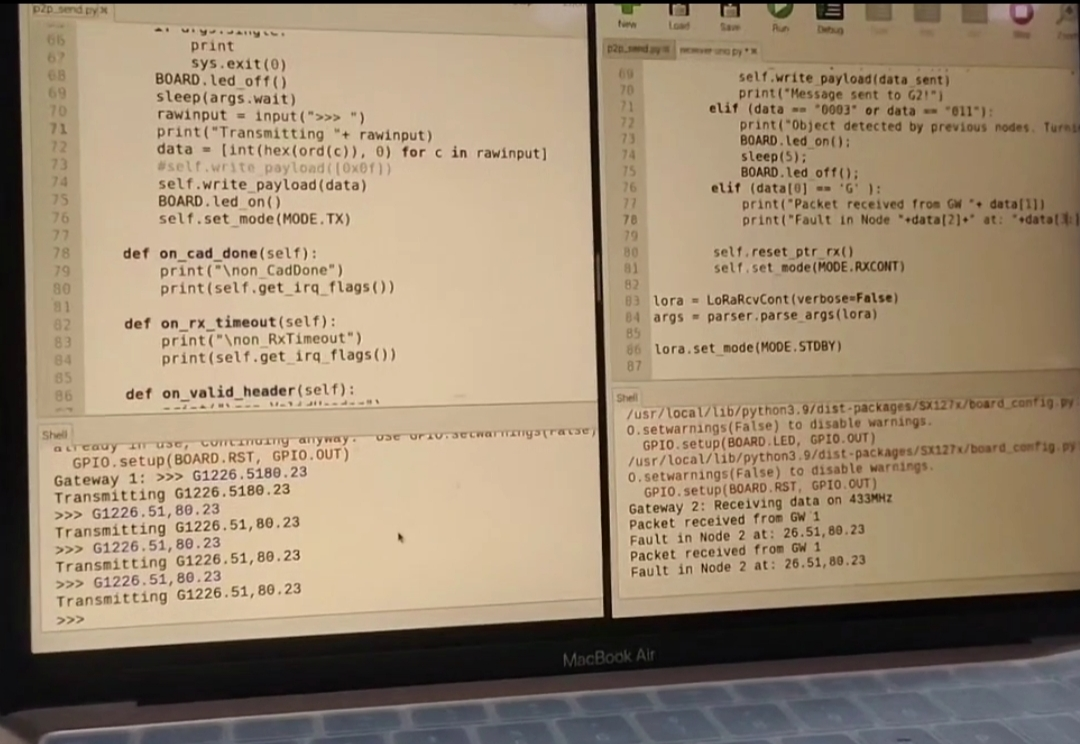
\includegraphics[width=0.5\textwidth]{images/module3-1.jpg}
  \caption{ The gateway receives the location of the faulty LED from nearby gateway. }
  \label{module3-1}
  \end{figure}
\end{enumerate}

\section{Discussion and Future Work}
This project was able to overcome the limitation of short-range communication provided by protocols such as Zigbee and BLE with the help of LoRa communication protocol. The number of sensor nodes is lesser in number as compared to other solutions which deploy sensors in every streetlight, as we consider 5 - 8 streetlights to be controlled by one node. The maintenance of the entire system becomes easier and faster due to real-time fault detection of nodes by using GPS modules installed at every node. The fault detection mechanism can be enhanced even further by using two LDR sensors for every streetlight - one sensor for sensing environmental light and the other for sensing the light from the streetlight. As of now the time of the day is detected on the basis of system time, i.e., 6 pm to 6 am is considered as night. The enhanced fault detection mechanism with two LDR sensors will be able to detect the time of the day without a time constraint and will work better in rainy/cloudy weather as well, where there can be the absence of environmental light even during the time period from 6 am to 6 pm. The other features that can be improved in the future are listed below:

\subsection{Localizing nodes without GPS}
Although having a GPS module equipped with IoT nodes provides ease of use and accuracy to us, it consumes a lot of power for the small energy-constrained IoT devices. Therefore, using the same technology for data communication as well as localization of the node will prove to be very advantageous. The localization of nodes can be achieved by analyzing the Time Difference of Arrival (TDoA) at the receiving gateway using techniques such as triangulation, multilateration, etc. The assumption is that the location of the gateway nodes is known beforehand (or is equipped with a GPS module), and other nodes localize themselves with respect to the gateway nodes.

A sensor node should send data to at least two gateway servers, where on the reception of data, the time of arrival of the packet is noted based on the system clocks of the gateways (the system clocks of all gateway servers should be synchronized). Based on the difference in the arrival time of the data packet on several gateway servers, the location of the transmitting sensor node is calculated. This technique is similar to collaborative multilateration. Interested readers can follow this for further information on this \cite{15} technique.

\subsection{Security}
In this project, the basic level of security was implemented by ensuring secure login in the gateway nodes and packet filtering in all nodes. Although it's a good start with the increasing digital security risk, the security of the IoT system can be further enhanced by including network segmentation using a firewall to keep any potential security threat outside the network. The Nagios or similar monitoring software can be used for real-time monitoring of the end nodes. IP and MAC binding of the gateways can be done to protect the system against MITM attacks, i.e., binding together the IP and MAC addresses so that any changes in either of them, makes the gateway node untrusted and all the communication to that gateway is stopped until the authenticity is re-established.

There are a few tradeoffs for this system as a whole. The fault repair by the repair team needs manual checking in an area of 500 - 600m, the area within a node group. Deploying this system in the existing network requires additional cabling between a group of streetlights for parallel connection. Another important factor is fault on a node. A fault on a node, unlike a fault on LED, will lead to the malfunctioning of multiple streetlights in its node group. This can be a challenge to the system and in the future, research can be on fault tolerance at the nodes without affecting the node group.


\section{Conclusion}
In this project, a smart street-lighting system is implemented using a two-tier architecture over the LoRa communication protocol. The proposed model is low-cost and scalable in its approach with respect to energy consumption and efficiency compared to the existing approaches. The model is easily deployable with the existing lighting system and particularly, the use of LoRa communication protocol overcomes the limitations of other currently used protocols such as ZigBee and BLE. The design also involves detecting faults in LEDs and sending this information immediately to the gateway, without disturbing the functioning of the remaining streetlights in that particular node group. The proposed system also takes care of cases where the information cannot be sent to the gateway, by sending it over Ethernet to the neighboring gateway directly. This automated system of node-to-node communication based on instantaneous communication and detection of the object was to aim for two things - cost-effectiveness and efficient energy consumption and both these were achieved through this project.


\section{Individual Contributions}
The individual contribution of each member of the project is listed in the table: \ref{tab: contribution}
\begin{table}[h]
\begin{center}
\begin{tabular}{ | m{8em} | m{22em}| m{6em} |} 

  \hline
  \textbf {Student Name} & \textbf{Contribution of work}  & \textbf {Percentage Contribution} \\
    \hline
    Deepak Mathur & LoRa communication sensor node to node, hardware integration, report preparation & 20\%\\
    \hline        
    Ashee Jain &  LoRa communication gateway to gateway, hardware integration, report preparation & 20\%\\
    \hline
    Srujana Sabbani & PIR and LDR sensor integration with node, hardware integration, report preparation & 20\%\\
    \hline
    Atanu Kar & LoRa communication sensor node to the gateway, hardware integration, PPT preparation & 20\%\\
    \hline
    Anjali Manoj & Integration of GPS module with node, hardware integration, report preparation & 20\%\\
    \hline
    \end{tabular}
    \caption{Individual contribution list}
    \label{tab: contribution}
\end{center}
\end{table}

\bibliography{references} 
\bibliographystyle{ieeetr}

\end{document}  